\documentclass[a4paper,10pt,twocolumn]{ltjarticle}
\usepackage{kaitoushu}

% グラフ用の共通スタイル定義
\pgfplotsset{
  myaxis/.style={
    axis lines=middle,
    xlabel={$x$}, ylabel={$y$},
    every axis x label/.style={at={(ticklabel* cs:1)},anchor=west},
    every axis y label/.style={at={(ticklabel* cs:1)},anchor=south},
    tick label style={font=\scriptsize},
    label style={font=\small},
    width=5.5cm, height=5cm,
    grid=none,
    samples=100,
  }
}

\begin{document}

\problemrange{3章：関数とグラフ — Check (p.38)（問180--188）}



\mondai{180}{次の関数について，偶関数か奇関数かを調べよ．}
\kotae{
(1) $2x$ → 奇\quad (2) $3x^{2}-1$ → 偶\quad (3) $x^{3}-x$ → 奇

(4) $\dfrac{x^{4}-1}{x^{2}}$ → 偶\quad (5) $3$ → 偶\quad (6) $3+x^{3}$ → どちらでもない
}

\mondai{181}{次の関数の定義域と値域を求めよ．}
\kotae{
(1) $y=\dfrac{3x-5}{x-2}=3+\dfrac{1}{x-2}$\quad 定義域$x\neq2$，値域$y\neq3$

(2) $y=-\sqrt{x+3}+4$\quad 定義域$x\geqq-3$，値域$y\leqq4$
}

\mondai{182}{$y=\dfrac{2}{x}$ を$x$方向に1，$y$方向に$-3$平行移動した関数を求めよ．}
\kotae{
$y=\dfrac{2}{x-1}-3$
}

\mondai{183}{$y=\sqrt{-x}$ を$x$方向に$-3$，$y$方向に2平行移動した関数を求めよ．}
\kotae{
$y=\sqrt{-x-3}+2$
}

\mondai{184}{次の関数のグラフをかけ．}
\kotae{
基本関数の平行移動で考える．

(1) $y=(x-1)^{3}-2$：変曲点$(1,-2)$

\begin{tikzpicture}
\begin{axis}[myaxis, xmin=-1.5,xmax=3.5,ymin=-5,ymax=5]
\addplot[thick,blue,domain=-1:3]{(x-1)^3-2};
\addplot[only marks,mark=*,mark size=1.5pt] coordinates {(1,-2)};
\end{axis}
\end{tikzpicture}

(2) $y=-(x+1)^{4}+1$：最大点$(-1,1)$

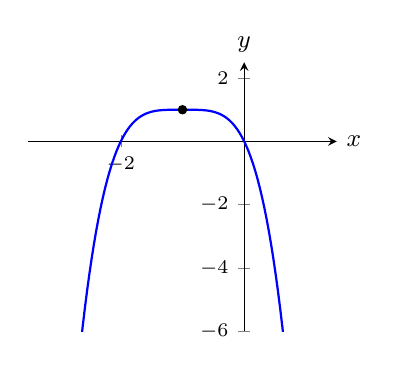
\begin{tikzpicture}
\begin{axis}[myaxis, xmin=-3.5,xmax=1.5,ymin=-6,ymax=2.5]
\addplot[thick,blue,domain=-2.8:0.8]{-(x+1)^4+1};
\addplot[only marks,mark=*,mark size=1.5pt] coordinates {(-1,1)};
\end{axis}
\end{tikzpicture}

(3) $y=\dfrac{1}{x+1}-2$：漸近線 $x=-1$，$y=-2$

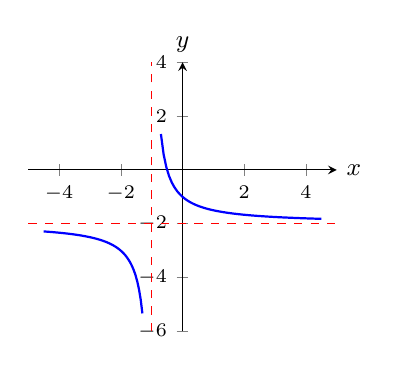
\begin{tikzpicture}
\begin{axis}[myaxis, xmin=-5,xmax=5,ymin=-6,ymax=4,
  restrict y to domain=-10:10]
\addplot[thick,blue,domain=-4.5:-1.3,samples=60]{1/(x+1)-2};
\addplot[thick,blue,domain=-0.7:4.5,samples=60]{1/(x+1)-2};
\addplot[dashed,red] coordinates {(-1,-6)(-1,4)};
\addplot[dashed,red] coordinates {(-5,-2)(5,-2)};
\end{axis}
\end{tikzpicture}

(4) $y=\dfrac{2x+3}{x+2}=2-\dfrac{1}{x+2}$：漸近線 $x=-2$，$y=2$

\begin{tikzpicture}
\begin{axis}[myaxis, xmin=-6,xmax=4,ymin=-4,ymax=8,
  restrict y to domain=-10:10]
\addplot[thick,blue,domain=-5.5:-2.3,samples=60]{(2*x+3)/(x+2)};
\addplot[thick,blue,domain=-1.7:3.5,samples=60]{(2*x+3)/(x+2)};
\addplot[dashed,red] coordinates {(-2,-4)(-2,8)};
\addplot[dashed,red] coordinates {(-6,2)(4,2)};
\end{axis}
\end{tikzpicture}

(5) $y=\sqrt{x+1}-2$：始点$(-1,-2)$

\begin{tikzpicture}
\begin{axis}[myaxis, xmin=-2,xmax=6,ymin=-3,ymax=2]
\addplot[thick,blue,domain=-1:5.5]{sqrt(x+1)-2};
\addplot[only marks,mark=*,mark size=1.5pt] coordinates {(-1,-2)};
\end{axis}
\end{tikzpicture}

(6) $y=\sqrt{-(x-1)}+1=\sqrt{1-x}+1$：始点$(1,1)$，$x\leqq1$

\begin{tikzpicture}
\begin{axis}[myaxis, xmin=-5,xmax=3,ymin=-1,ymax=4]
\addplot[thick,blue,domain=-4.5:1]{sqrt(1-x)+1};
\addplot[only marks,mark=*,mark size=1.5pt] coordinates {(1,1)};
\end{axis}
\end{tikzpicture}
}

\mondai{185}{$y=3x^{4}-2x$ の$y$軸対称 → $y=3x^{4}+2x$}
\kotae{
$x\to-x$：$y=3(-x)^{4}-2(-x)=3x^{4}+2x$
}

\mondai{186}{$y=\sqrt{x+1}-1$ の原点対称 → $y=1-\sqrt{1-x}$}
\kotae{
$x\to-x$，$y\to-y$：$-y=\sqrt{-x+1}-1$ → $y=1-\sqrt{1-x}$
}

\mondai{187}{$y=\dfrac{3}{x+2}$ の逆関数を求めよ．}
\kotae{
$x=\dfrac{3}{y}-2$，入替えて $y=\dfrac{3}{x}-2$

定義域$x\neq0$，値域$y\neq-2$
}

\mondai{188}{$f(x)=(x-2)^{2}\;(x\leqq2)$ について答えよ．}
\kotae{
(1) $x-2=-\sqrt{y}$，$x=2-\sqrt{y}$．入替えて $g(x)=2-\sqrt{x}\;(x\geqq0)$

(2) 交点は $y=x$ 上．$(x-2)^{2}=x$，$(x-1)(x-4)=0$

$x\leqq2$ より $x=1$ → 交点$(1,1)$
}

\end{document}
